\documentclass[border=4pt]{standalone}
\usepackage{tikz}
\usetikzlibrary{positioning, arrows.meta, shapes.geometric, calc, fit, backgrounds}
\usepackage{amsmath,amssymb}

\begin{document}
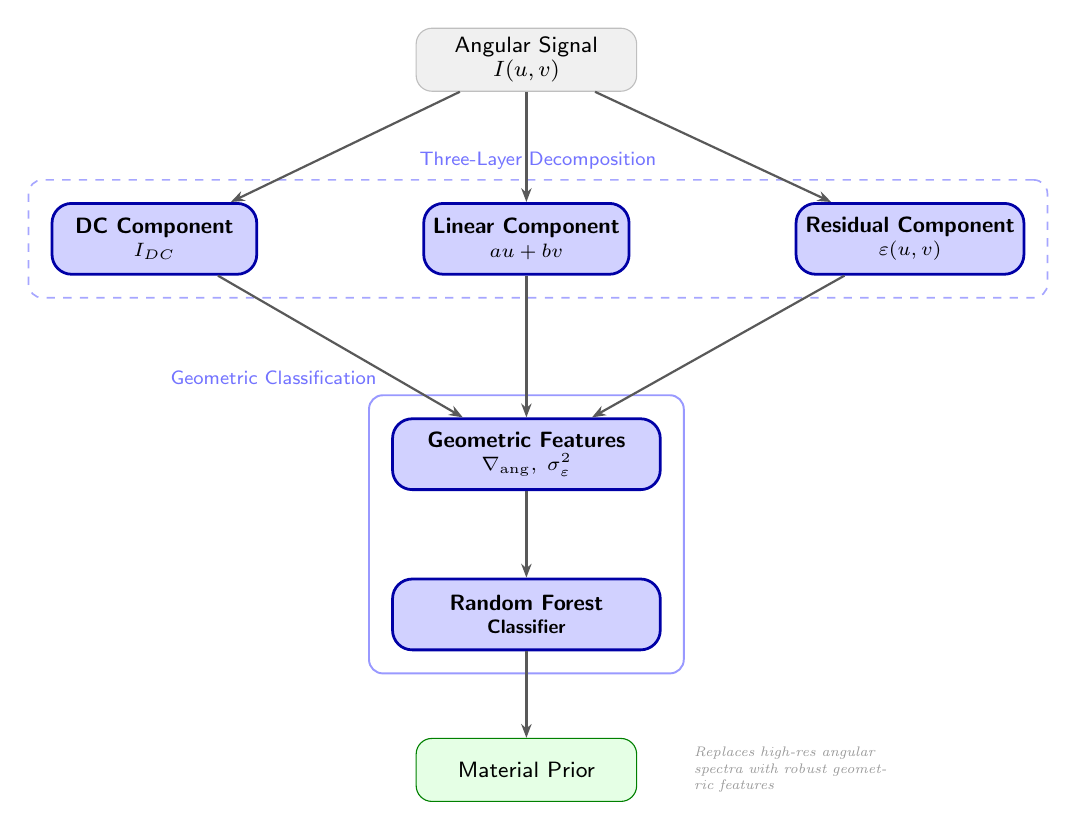
\begin{tikzpicture}[
  input/.style={draw, rounded corners=2mm, minimum width=2.8cm, minimum height=0.8cm,
                fill=gray!12, draw=gray!50, align=center,
                font=\sffamily\footnotesize},
  innov/.style={draw, rounded corners=2.5mm, minimum width=2.6cm, minimum height=0.9cm,
                fill=blue!18, draw=blue!65!black, line width=1pt, align=center,
                font=\sffamily\footnotesize\bfseries},
  innov_wide/.style={draw, rounded corners=2.5mm, minimum width=3.4cm, minimum height=0.9cm,
                fill=blue!18, draw=blue!65!black, line width=1pt, align=center,
                font=\sffamily\footnotesize\bfseries},
  output/.style={draw, rounded corners=2mm, minimum width=2.8cm, minimum height=0.8cm,
                 fill=green!10, draw=green!50!black, align=center,
                 font=\sffamily\footnotesize},
  arr/.style={-{Stealth[length=5pt]}, thick, color=black!65},
  gbox_dashed/.style={draw=blue!35, dashed, rounded corners=5pt, inner sep=8pt, line width=0.6pt},
  gbox_solid/.style={draw=blue!40, solid, rounded corners=5pt, inner sep=8pt, line width=0.7pt},
  lbl/.style={font=\sffamily\scriptsize, text=black!50},
]

% Input
\node[input] (m1) {Angular Signal\\[-1pt]$I(u,v)$};

% Three decomposition components
\node[innov, below left=1.4cm and 2.0cm of m1] (m2)
  {DC Component\\[-1pt]{\scriptsize$I_{DC}$}};
\node[innov, below=1.4cm of m1] (m3)
  {Linear Component\\[-1pt]{\scriptsize$au + bv$}};
\node[innov, below right=1.4cm and 2.0cm of m1] (m4)
  {Residual Component\\[-1pt]{\scriptsize$\varepsilon(u,v)$}};

% Geometric Features
\node[innov_wide, below=1.8cm of m3] (m5)
  {Geometric Features\\[-1pt]{\scriptsize$\nabla_{\mathrm{ang}},\;\sigma_\varepsilon^2$}};

% Random Forest
\node[innov_wide, below=1.1cm of m5] (m6)
  {Random Forest\\[-1pt]{\scriptsize Classifier}};

% Output
\node[output, below=1.1cm of m6] (m7)
  {Material Prior};

% Arrows
\draw[arr] (m1) -- (m2);
\draw[arr] (m1) -- (m3);
\draw[arr] (m1) -- (m4);
\draw[arr] (m2) -- (m5);
\draw[arr] (m3) -- (m5);
\draw[arr] (m4) -- (m5);
\draw[arr] (m5) -- (m6);
\draw[arr] (m6) -- (m7);

% Group boxes on background
\begin{scope}[on background layer]
  \node[gbox_dashed, fit=(m2)(m3)(m4),
        label={[font=\sffamily\scriptsize, text=blue!55]above:Three-Layer Decomposition}] {};
  \node[gbox_solid, fit=(m5)(m6),
        label={[font=\sffamily\scriptsize, text=blue!55]above left:Geometric Classification}] {};
\end{scope}

% Annotation
\node[right=0.6cm of m7, font=\tiny\itshape, text=black!40, text width=2.8cm, align=left]
  {Replaces high-res angular spectra with robust geometric features};

\end{tikzpicture}
\end{document}